\documentclass{beamer}
%\setbeameroption{show only notes}
\usepackage{polyglossia}
\usetheme{default} %minimal
\setbeamercovered{transparent}
\setbeamertemplate{bibliography item}{}
\setbeamertemplate{caption}[numbered]
\setbeamercolor*{bibliography entry title}{fg=black}
\setbeamercolor*{bibliography entry author}{fg=black}
\setbeamercolor*{bibliography entry location}{fg=black}
\setbeamercolor*{bibliography entry note}{fg=black}
\usepackage{natbib}
\bibliographystyle{plain}
\renewcommand\bibfont{\scriptsize}
\beamertemplatenavigationsymbolsempty

\AtBeginSection[]
{
  \begin{frame}<beamer>
    \frametitle{Outline}
    \tableofcontents[currentsection]
  \end{frame}
}


\title{Robust Information-theoretic Clustering}
\subtitle{}

\author{Simon Lackerbauer}

\institute[Ludwig-Maximilians-Universität München]
{
  Institut für Informatik\\
  Ludwig-Maximilians-Universität München\\
  lackerbauer@lrz.mwn.de
}

\date{Seminar \textit{Information Theoretic Data Mining} im WS 2015/16}

\subject{}

\AtBeginSubsection[]
{
  \begin{frame}<beamer>{Outline}
    \tableofcontents[currentsection,currentsubsection]
  \end{frame}
}


\begin{document}
  
  \begin{frame}
    \titlepage
  \end{frame}
  
  \note{Guten Morgen, mein Name ist Simon Lackerbauer und ich trage heute vor über einen auf der SIGKDD 2006 vorgestellten Algorithmus zum automatisierten Clustering vor.}
  
  \begin{frame}{Outline}
    \tableofcontents
  \end{frame}
  
  \note{Hier ist mal der grobe Aufbau: Zuerst schaun wir uns das Problem anhand einiger einfacher Beispiele an, danach erkläre ich das RIC framework und seine einzelnen Bestandteile - Volume after Compression, Robust Fitting und Cluster Merging, die erst im Zusammenspiel miteinander tatsächlich in der Lage sind, das Problem anzugehen.\\Danach sehen wir uns noch einige reale Daten an, die der Algorithmus geclustered hat und gehen kurz auf Vergleiche mit traditionellen Algorithmen ein.}
  
  \section{Clustering Problems}
  
  \note{Gut, also erstmal ab zum Problem - oder besser gesagt den Problemen.}
  
  \begin{frame}{Clustering Problems}{}
    \begin{itemize}
      \item There exist a wide range of possible clustering algorithms.
      \item Many need user input or assume only Gaussian clusters
      \item We want an algorithm without user input that automatically selects appropriate cluster functions
    \end{itemize}
  \end{frame}
  
  \note{Das Problem (Daten zu sinnvoll in Cluster zu packen) an sich ist natürlich nicht neu. Ein Cluster ist nichts anderes als eine Anhäufung von Datenpunkten nach einem bestimmten Muster, bzw. nach einer bestimmten Verteilungsfunktion. Datenpunkte innerhalb so eines Clusters sind nicht unabhängig von der zugrundeliegenden Verteilung: Wenn man weiß, wie die Daten geclustered sind, kann man also vielleicht interessante Zusammenhänge in den Daten einfach erkennen.\\Das bedeutet natürlich auch, dass sich da schon mehrere Leute Gedanken drüber gemacht haben. K-means als immernoch sehr weit verbreiteter, recht einfacher Algorithmus, beispielsweise geht bis auf die 50er Jahre zurück.}
  
  \note{K-means ist nicht der einzige solche Algorithmus, aber dient gut als Beispiel für alle Probleme, die es im Allgemeinen gibt. Man braucht einen Eingabewert (die Zahl der vorhandenen Cluster), was natürlich ein bisschen das Problem verschleiert, denn woher soll man das idR wissen? Danach haben dann alle Cluster (wenn man sich Daten in 2D anschaut) so ellipsenhafte Formen, weil der Algorithmus eine Gauss-Verteilung annimmt - und gerade das machen viele herkömmliche Algorithmen.\\Man will also einen Algorithmus, der ohne Input auskommt und zusätzlich unabhängig ist in der Auswahl der Dichtefunktion, auf der der Cluster basiert.}
  
  \begin{frame}{Clustering Problems}{Example: How not to do it}
    \begin{figure}
      \centering
      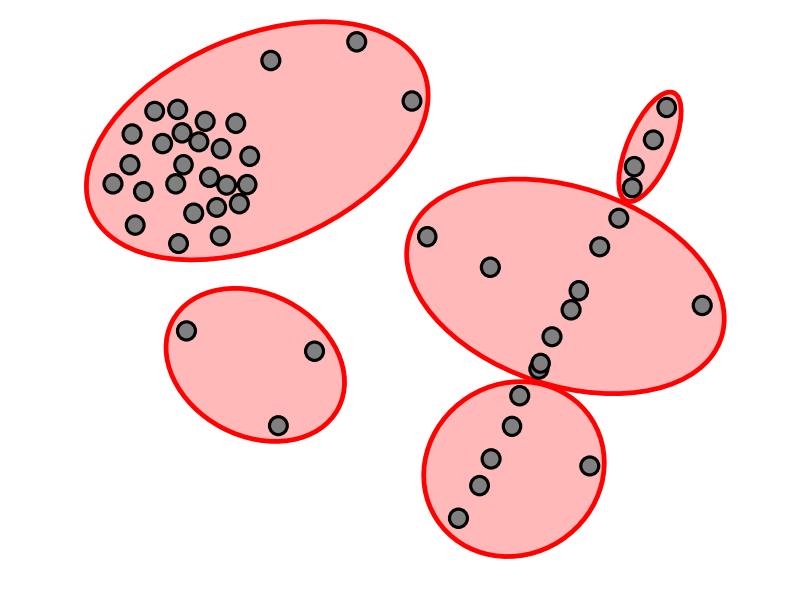
\includegraphics[width=0.7\linewidth]{imgs/bad_clustering}
      \caption[]{Example of “Bad” Clustering\cite{Bohm2006-ts}}
      \label{fig:bad_clustering}
    \end{figure}    
  \end{frame}
  
  \note{Hier sieht man ein Beispiel, was möglicherweise ein K-Means gefunden hätte, wenn man als Input 5 eingibt. Bei Input zwei wären wahrscheinlich diese zwei Gruppen rausgekommen usw. Man sieht gleich, dass ein weiteres großen Problem die Outlier-Behandlung ist. Der schlechte Algorithmus ist nicht robust und versucht auf Teufel komm raus, Noise in die Cluster reinzupacken.}
  
  \begin{frame}{Clustering Problems}{Example: Reasonable reduction}
    \begin{figure}
      \centering
      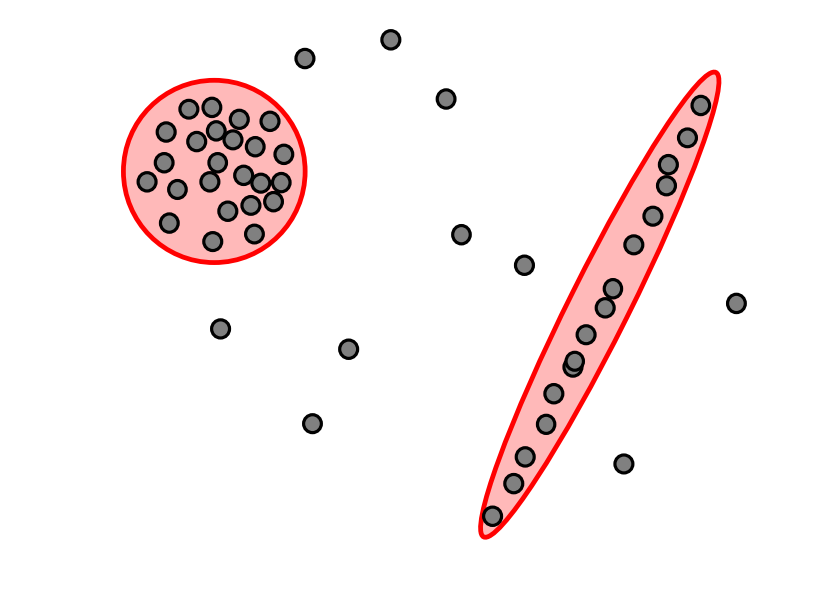
\includegraphics[width=0.7\linewidth]{imgs/good_clustering}
      \caption[]{Example of “Good” Clustering\cite{Bohm2006-ts}}
      \label{fig:good_clustering}
    \end{figure}    
  \end{frame}
  
  \note{So dagegen macht das ganze gleich viel mehr Sinn. Ein auf beiden Axen normalverteilter Cluster und ein korrelierter, linienförmiger Cluster. Und dazwischen ein paar Noise-Punkte, die ignoriert werden.}
  
  \begin{frame}{Comparison of examples}{}
    \textbf{What makes the second pattern better than the first?}
    \begin{itemize}
      \item It's more descriptive of the interesting patterns in the data, because outliers have been “omitted”.
      \item The clusters in the “good” example are those a human would immediately recognize as points being associated somehow.
    \end{itemize}
  \end{frame}
  
  \note{Man kann das auch etwas formaler ausdrücken und sagen, dass die zwei guten Cluster die Daten schlicht besser beschreiben. Nur aus der Form und Lage der Cluster allein lässt sich Information ableiten, was bei dem schlechten Beispiel nicht der Fall ist. Hier, im einfachen 2D-Beispiel deckt sich das natürlich mit den Clustern, die auch ein Mensch intuitiv eingezeichnen hätte. Aber es gibt natürlich Datensets, wo auch der Mensch nicht auf Anhieb sofort was sieht (beispielsweise das Set ganz am Ende) und demnach nicht dem Algorithmus mit Intuition "helfen" kann.}
  
  \begin{frame}{Measuring Success}{}
        This human intuition must be translated into a dependable clustering algorithm, for which two measures for success can be defined:
        \begin{itemize}
          \item \uncover<2->{\textbf{Goodness of fit}}
          \item \uncover<3->{\textbf{Efficiency}}     
        \end{itemize}
  \end{frame}
  
  \note{Wir wollen also einen Algorithmus, der zwei Voraussetzungen erfüllt: Goodness of fit: Wie gut passt der cluster tatsächlich zu den Daten? Bzw. Formal: wie kriegt man eine funktion, die ein scoring von Clustern zulässt und einen "guten" Score für das zweite Beispiel oben ausspricht und einen "schlechten" für die noisy cluster aus dem schlechten Beispiel?}
  
  \note{Wie kriegt man das mit ordentlicher Laufzeit hin und ohne, dass man von Outliers/Noise zu sehr gestört wird?}
  
  \section{Solution: The iterative approach}
  
  \note{gut, also jetzt ab ins eigentliche Thema}
  
  \subsection{VAC -- Volume After Compression}
  
  \note{Fangen wir an mit dem wohl wichtigsten Subalgorithmus: Volume After Compression}
  
  \begin{frame}{Proposition for a solution: VAC}{}
    \textbf{VAC - Volume after Compression}\\
    \begin{itemize}
      \item does not specify good grouping
      \item specifies for two groupings $x,y$ which one is better (e.g., because $VAC(x) < VAC(y) \rightarrow$ x is a better grouping)
      \item size of total, \textbf{lossless} compression
    \end{itemize}
  \end{frame}
  
  \note{Das VAC-Kriterion ist ein informationstheretischer Ansatz des Scorings. Je besser man die Daten beschreibt, desto besser kann man diese auch ohne Verlust von Information komprimieren. Genauso wie ich stark komprimiert mit dem Wort "Integer" die ganzen Zahlen beschreiben kann, ohne die alle Aufzählen zu müssen, beschreibt ein guter Cluster die darunter liegenden Daten, ohne jeden Datenpunkt einzeln aufzählen zu müssen.\\Wichtig dabei: das VAC beschreibt keinen absoluten Score. Man kann nicht zwischen zwei Datensets die VAC scores vergleichen, und dann sagen, dass mit dem niedrigeren Score ist besser geclustert. Man kann aber innerhalb des selben Datensets zwei mögliche Clusterings vergleichen und dann eindeutig sagen: Das mit dem niedrigeren Score beschreibt die Daten einfach besser, denn es braucht weniger Informationstransfer, um das gleiche Wissen auf beiden Seiten herzustellen.}
  
  \begin{frame}{Proposition for a solution: VAC}{Integer Encoding}
    \begin{itemize}
      \item point coordinates are always integers
      \item self-delimiting encoding of integers: Elias (gamma) codes
      \item smaller integers require fewer bytes
    \end{itemize}
  \end{frame}
  
  \note{Wenn man jetzt anfängt, die Daten vorzubereiten, gehen wir davon aus, dass alle Koordinaten integer sind (weil man sowieso endliche Präzision nur darstellen kann) und können demnach die Achsten in ein "Grid" einteilen - man kann das Grid aber natürlich beliebig präzise machen. Integer kann man via Elias encoding ohne jegliches Padding eindeutig encoden, so dass kleine Zahlen weniger Platz verbrauchen - das ist später wichtig.}

  \begin{frame}{Proposition for a solution: VAC}{Cluster Encoding}
    \begin{itemize}
      \item uses Huffman encoding for positioning points with probability distribution according to assumed cluster pdf
      \item such, if we assume the correct distribution for the cluster, core points will be more efficiently encoded
    \end{itemize}
  \end{frame}
  
  \note{Huffman encoding geben uns für alle Koordinaten eines Punktes einen bit-string $l = log_2(1/P(x))$, so dass Punkte die an einem Punkt liegen, wo die Wahrscheinlichkeit laut pdf höher ist, dass sie liegen, weniger Bits verbrauchen als solche, die weiter am Rand der Verteilung liegen. Je besser demnach unsere Annahme der Distribution für ein Cluster ist, desto effectiver lassen sich die Punkte kodieren.}
  
  \begin{frame}{Proposition for a solution: VAC}{Cluster Encoding}
    \begin{figure}
      \centering
      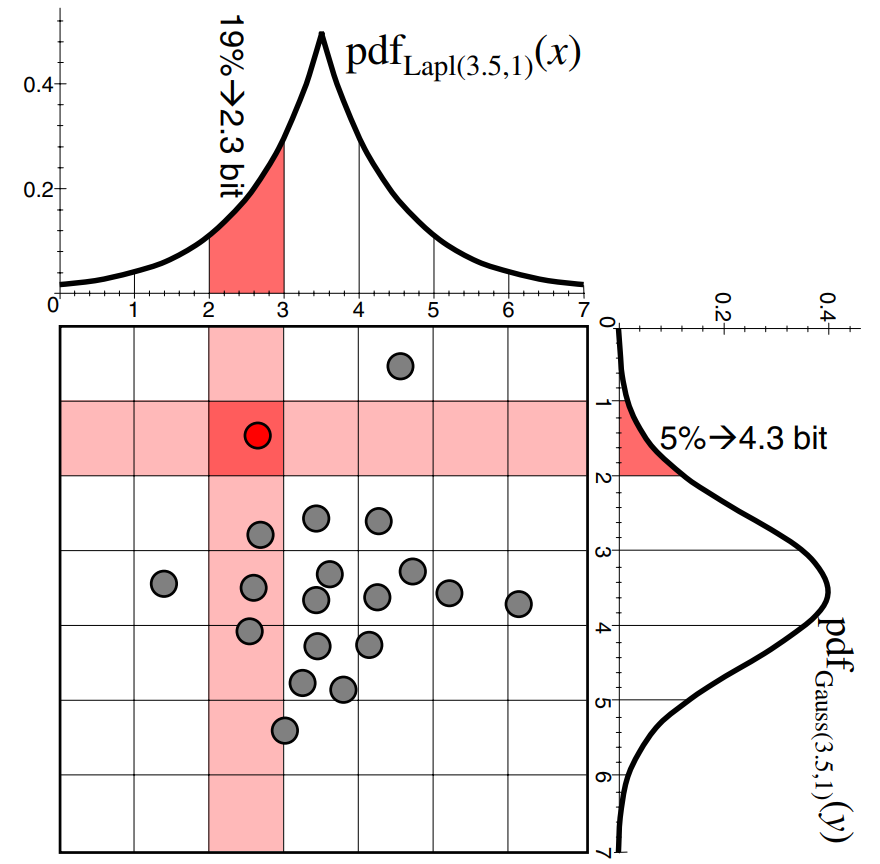
\includegraphics[width=0.65\linewidth]{imgs/vac}
      \caption[]{Example of VAC\cite{Bohm2006-ts}}
      \label{fig:vac}
    \end{figure}    
  \end{frame}
  
  \note{Hier sieht man ein Beispiel der Aufteilung eines Datensets in ein Grid, und dann die Enkodierung der Koordinaten. Man sieht gut, wie bei beiden Verteilungen das Gros der Punkte direkt in der Mitte der jeweiligen Dichtefunktion liegt.}
  
  \begin{frame}{Proposition for a solution: VAC}{Cluster encoding}
    \begin{definition}[VAC of point $\vec{x}$]
      Let $\vec{x} \in \mathbb{R}^d$ be a point of a cluster $C$ and $\overrightarrow{pdf}(\vec{x})$ be a $d$-dimensional vector of probability density functions  which are associated to $C$. Each $pdf_i(x_i)$ is selected from  a set of predefined probability density functions with corresponding parameters, i.e. $PDF = \{pdf_{Gauss(\mu_i, \sigma_i)}, pdf_{uniform(lb_i, ub_i)}, pdf_{Lapl(a_i, b_i)}, ...\}$, $\mu_i, lb_i, ub_i, a_i \in \mathbb{R}, \sigma_i, b_i \in \mathbb{R}^+$. Let $\gamma$ be the grid constant (distance between grid cells). The $VAC_i$ of coordinate $i$ of point $\vec{x}$ corresponds to
      \[VAC_i(x) = \log_2 \frac{1}{pdf_i(x_i) \cdot \gamma}\]
      The $VAC$ of point $\vec{x}$ corresponds to
      \[VAC(x) = \left( \log_2 \frac{n}{|C|}\right) + \sum_{0 \leq i < d} VAC_i(x)\]
    \end{definition}
  \end{frame}
  
  \note{Hier nochmal eine formale Definition des VAC-Kriteriums. wichtig ist vA, dass die möglichen PDFs vorher schon festgelegt sind und dann via ID angesprochen werden können.}
  
  \begin{frame}{Proposition for a solution: VAC}{Cluster Encoding and Decorrelation}
    \begin{itemize}
      \item $\gamma$ is a measure of granularity of grid cells
      \item absolute VAC changes with grid resolution, but relative VAC stays the same
      \item to choose optimal parameter settings for clusters, we use the statistical parameter of the dataset
      \item if data is correlated amongst itself, define a decorrelation matrix iff the VAC savings at least compensate for saving the decorrelation matrix
    \end{itemize}
  \end{frame}
  
  \subsection{RF -- Robust Fitting}
  
  \note{Um mithilfe des VAC Kriterions jetzt tatsächlich Cluster beschreiben zu können, brauchen wir noch 2 Algorithmen, die bei der tatsächlichen erstellung von Clustern helfen. Einer davon ist Robust Fitting.}
  
  \begin{frame}{Two helper algorithms}{Robust Fitting}
    \begin{itemize}
      \item Start: get as input a set of clusters $\mathcal{C} = \{C_1,...,C_k\}$ by an arbitrary method
      \item for every $C_i$ in $\mathcal{C}$ define a similarity measure (decorrelation matrix == ellipsoid)
      \item use the VAC score to try out decorrelation matrices until the one with the lowest VAC is found 
    \end{itemize}
  \end{frame}
 
  \note{RF ist an sich recht einfach zu beschreiben - man kriegt erstmal irgendeine Anzahl von Clustern nach irgendeiner Methode (da kann man auch erstmal K-means nehmen). Dann nimmt man sich eine decorrelation matrix, die einen Ellipsoid beschreibt, der die Grenze zwischen Core points und Outliers darstellt. Dann probiert man verschiedene Grenzen durch, bis man diejenige gefunden hat, die den niedrigsten VAC-Score produziert. (Da jeder Cluster nur endlich viele Punkte hat, kann man da tatsáchlich alle Punkte von innen nach außen nacheinander durchprobieren.)}
  
  \begin{frame}{Two helper algorithms}{Robust Fitting}
    Decorrelation Matrix:
    \begin{itemize}
      \item contains the vectors that define the space in which points in the cluster reside
      \item to improve robustness of cluster center estimation use coordination-wise median instead of arithmetic means
      \item of the several matrices generated during this step, again partition into core points and noise by choosing the one with best VAC
    \end{itemize}    
  \end{frame}
  
  \note{}
  
  \begin{frame}{Two helper algorithms}{Robust Fitting}
    \begin{figure}
      \centering
      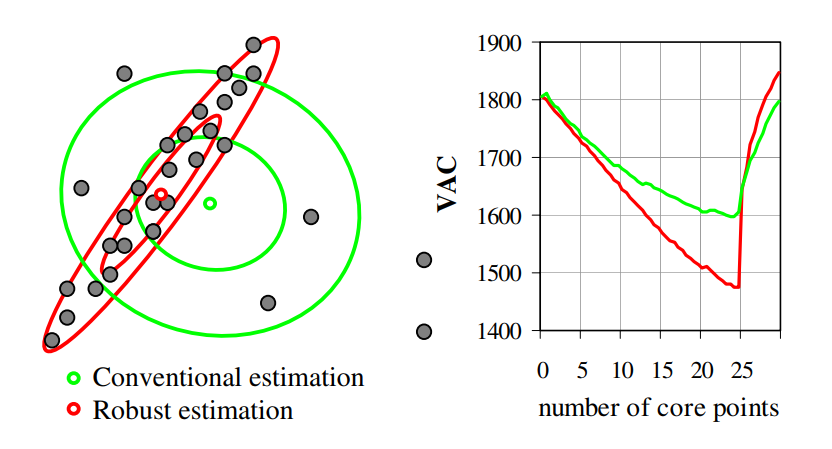
\includegraphics[width=\linewidth]{imgs/robust_estimation}
      \caption[]{Conventional and robust estimation\cite{Bohm2006-ts}}
      \label{fig:robust_estimation}
    \end{figure}    
  \end{frame}
  
  \note{}
  
  \subsection{CM -- Cluster Merging}
  
  \begin{frame}{Two helper algorithms}{Cluster Merging}
    \begin{itemize}
      \item Start: get as input a set of clusters $\mathcal{C} = \{C_1,...,C_k\}$ by an arbitrary method
      \item Purify (of noise) each cluster individually
    \end{itemize}    
  \end{frame}
  
  \note{}

  \begin{frame}{Two helper algorithms}{Cluster Merging}
    \begin{figure}
      \centering
      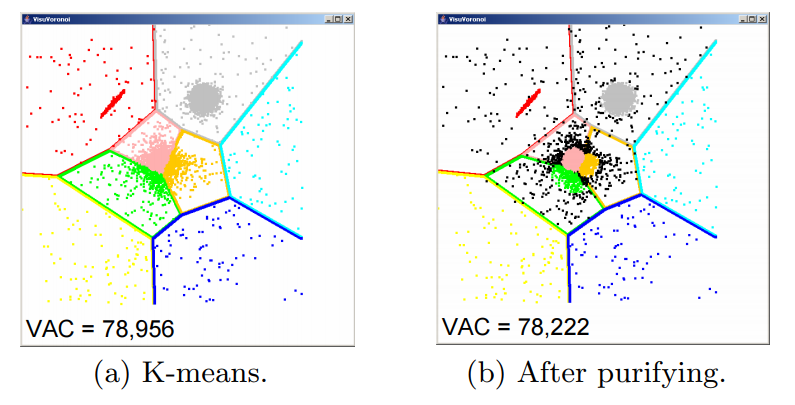
\includegraphics[width=\linewidth]{imgs/cluster_merging1}
      \caption[]{Clustering by using K-means and then purifying\cite{Bohm2006-ts}}
      \label{fig:cluster_merging1}
    \end{figure}    
  \end{frame}
  
  \note{}
  
  \begin{frame}{Two helper algorithms}{Cluster Merging}
    \begin{figure}
      \centering
      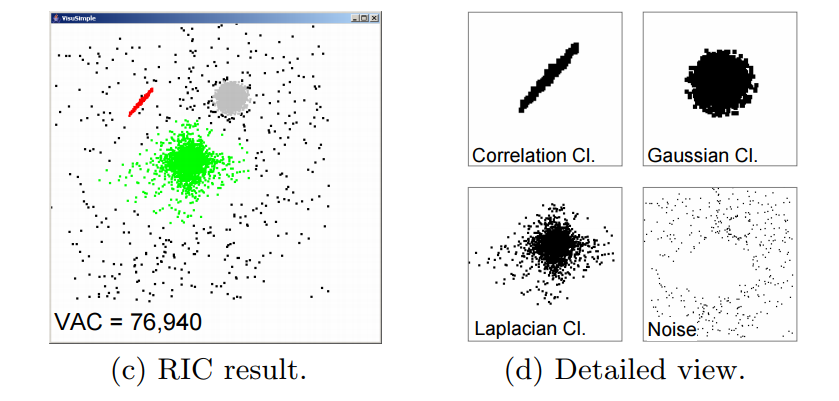
\includegraphics[width=\linewidth]{imgs/cluster_merging2}
      \caption[]{After merging\cite{Bohm2006-ts}}
      \label{fig:cluster_merging2}
    \end{figure}    
  \end{frame}
  
  \note{}
  
  \section{Example: Cat Retina Images}
  
  \begin{frame}{Example: Cat Retina Images}{}
    \begin{itemize}
      \item 219 blocks of retinal images, 96 tiles per image $\rightarrow$ 22,024 tiles in total (example tiles in figure \ref{fig:cat5})
      \item each tile is represented as vector of 7 features (figure \ref{fig:cat1}(a))
      \item RIC finds 13 clusters, color coded in figure \ref{fig:cat1}(b)
      \item Example clusters in figures \ref{fig:cat2}(a)-(f)
    \end{itemize}
  \end{frame}
  
  \note{}
  
  \begin{frame}{Example: Cat Retina Images}{}
    \begin{figure}
      \centering
      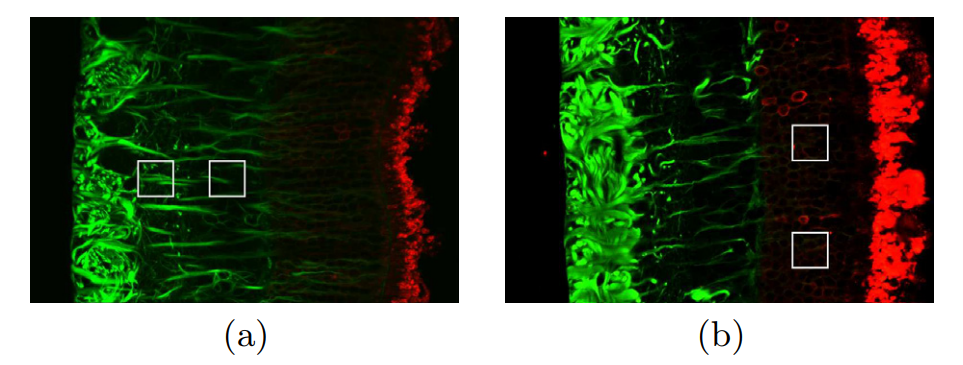
\includegraphics[width=\linewidth]{imgs/cat5}
      \caption[]{Examples of tiles\cite{Bohm2006-ts}}
      \label{fig:cat5}
    \end{figure}    
  \end{frame}
  
  \note{}
  
  \begin{frame}{Example: Cat Retina Images}{}
    \begin{figure}
      \centering
      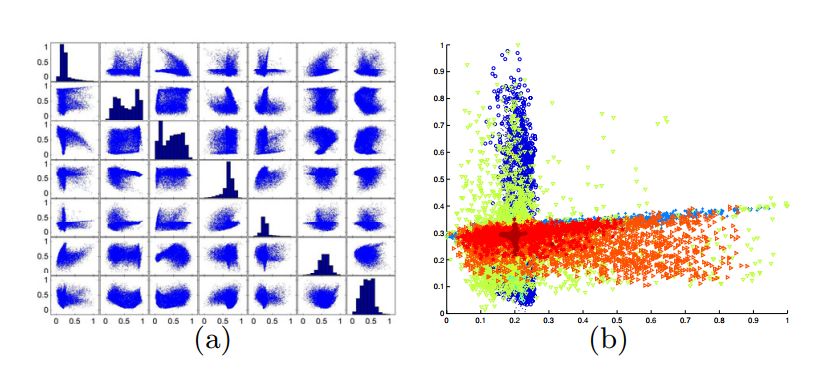
\includegraphics[width=\linewidth]{imgs/cat1}
      \caption[]{Visualization of cat retina data\cite{Bohm2006-ts}}
      \label{fig:cat1}
    \end{figure}    
  \end{frame}
  
  \note{}
  
  \begin{frame}{Example: Cat Retina Images}{}
    \begin{figure}
      \centering
      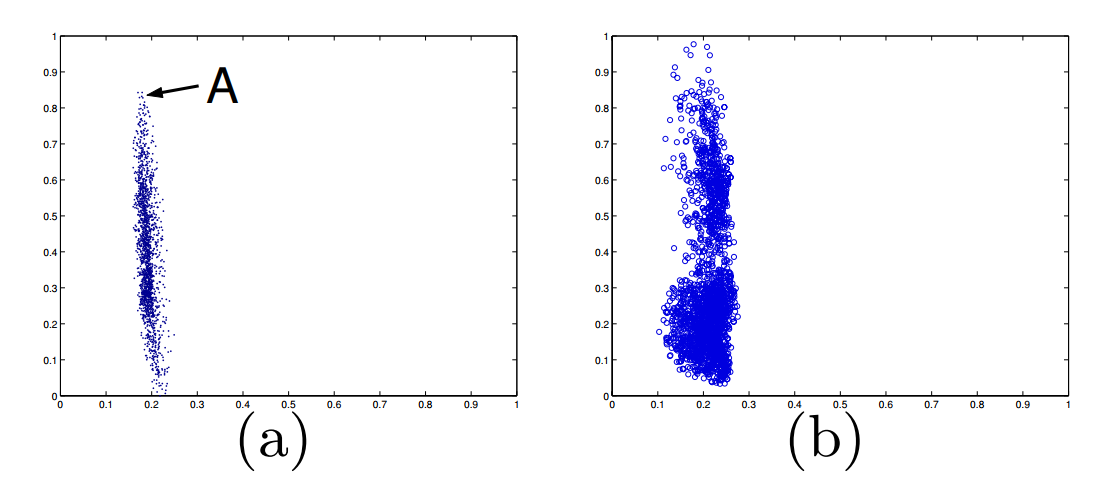
\includegraphics[width=\linewidth]{imgs/cat2}
      \caption[]{Example clusters\cite{Bohm2006-ts}}
      \label{fig:cat2}
    \end{figure}    
  \end{frame}
  
  \note{}
  
  \setcounter{figure}{7}
  
  \begin{frame}{Example: Cat Retina Images}{}
    \begin{figure}
      \centering
      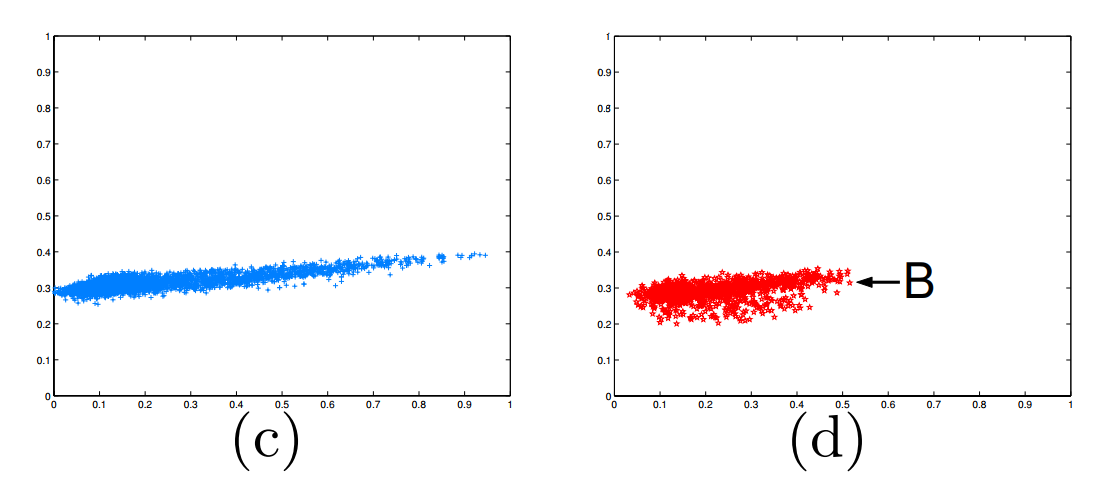
\includegraphics[width=\linewidth]{imgs/cat3}
      \caption[]{Example clusters\cite{Bohm2006-ts}}
      \label{fig:cat3}
    \end{figure}    
  \end{frame}
  
  \note{}
  
  \setcounter{figure}{7}
  
  \begin{frame}{Example: Cat Retina Images}{}
    \begin{figure}
      \centering
      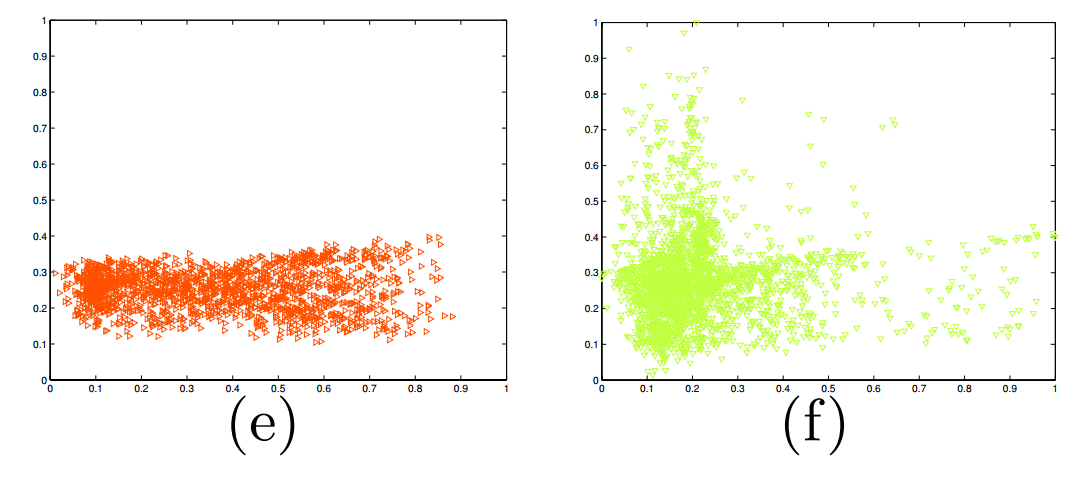
\includegraphics[width=\linewidth]{imgs/cat4}
      \caption[]{Example clusters\cite{Bohm2006-ts}}
      \label{fig:cat4}
    \end{figure}    
  \end{frame}
  
  \note{}
  
  \section{Summary}
  
  \begin{frame}{Summary}
    \begin{itemize}
      \item The VAC criterion provides a \alert{stable measure of goodness of fit}.
      \item The RIC framework is very flexible, does not rely on user input and can handle any distribution that can be described by a pdf
      \item Anytime a new, better clustering algorithm is introduced, RIC can improve on it by running its parts (CM and RF) with the better algorithm as a starting point\\
    \end{itemize}
  \end{frame}
  
  \note{Vielen Dank für Eure Aufmerksamkeit!}
  
  \section{References}
  
  \begin{frame}[t]{References}
    \bibliography{sources}
  \end{frame}
  
\end{document}
